\documentclass[a4paper, oneside 12pt]{article}
\usepackage{amsmath} % http://ctan.org/pkg/amsmath
\usepackage{graphicx}
\usepackage{caption}
\usepackage{subcaption}
\usepackage{scrextend}

\begin{document}
	
\title{3rd Year Plasma Lab Report}	
\author{Examination number : Y1468665 \\ University of York}
\maketitle

\begin{addmargin}[-3em]{-3em}

\section*{Abstract}
\textbf{ A molecular system was using values typical of a syatem of Argon fluid.}


\newpage
\section{Introduction}

Molecular dynamics we can investigate the constant volume (isometric) heat capacity and see how it reponded to changes in temperature.

A molecular simulation is a deterministic system, as we can solve the equation of motion for the particle if we know the potential. We simulate an isolated system as the NVE the number of particles and the total energy is conserved. An isolated system is impossible to measure experimentally as the act of measuring it destroys the isolation of the system. 

The main factor in producing accurate and physical results from a molecular dynamics simulation is the choice of potential that is chosen to describe the system. It is important for all experiments to be compared to experimental data to validate the assumptions made in the model. The LJ is a widely used potential for atoms, therefore it is expected that the results from this experiment should agree with experimental data. 

The Lennard-Jones (LJ) potential is at the heart of the system that was investigated here. The potential is still a good model for Argon. T*=1 is 120k for Argon. we want to be able to measure the specific heat capacity of a material. The LJ has a $\frac{1}{r^6}$ which means it has an infinite range. 

A molecular dynamics simulation writes out easily obtainable properties of the system.


The thermodynamic limit.


NVT or NVE great canonical ensemble 

DFT 

Molecular dynamics problems take a long time to run. It becomes more practical to use modular programs. A shell script was used to set up the initial condition for the system, this initial configuration was used to simulate the system. 

stratified sampling, systematic the same element from each block or random sampling. Block averaging converges to the true standard deviation quicker, with a smaller block length.

Reduced units are often used in molecular dynamics. 

The system starts in an unphysical state which is generated from the crystal.f90 program. Equilibration state runs the system at constant temperature, a canonical ensemble, NVT system. This is more computationally expensive but effectively ‘melts’ the lattice structure generated which is more representative of a solid.   


\newpage
\section{Theory}

Lennard-Jones potential is used infinite range though the largest term is a $^{-6}$ dependence. This means the potential can be truncated after a certain distance. There is a long range potential to deal with this which assumes the sea of particles produce a mean field approximation. 

The LJ potential is of the form:
\begin{equation}
	u^{LJ}(r)  = 4 \epsilon \left[ \left( \frac{\sigma}{r} \right)^{12} -  \left( \frac{\sigma}{r} \right)^6\right]
\end{equation}


Thermodynamic response functions, properties that are related to changes in temperature . The specific heat of a fluid can be obtained from the gradient of the Internal energy of the system as a function of temperature. This was the first method used,

The configurational internal energy requires multiple temperatures simulated as we need a function to differentiate to find $C_v$. This method is simpler however is computationally more expensive as it requires the simulation to be run for many temperatures.

Fluctuation formula uses the theory of statistical mechanics $C_v$ can be estimated from one trajectory. This method requires data analysis. 
\begin{equation}
	C_v^* = \frac{3}{2} \left[ 1 - \frac{2}{3 N T^{*2}} \left< ( \delta E^*_k)^2 \right> \right] ^{-1}
\end{equation}
Where 
\begin{equation}
	\left< ( \delta E^*_k)^2 \right> = \left< ( E^*_k)^2 \right> - \left< E^*_k \right>^2
\end{equation}

The standard deviation in the mean provides an estimate for the size of an error in a measurement. The crucial part is that each measurement is assumed to be independent of the other measurements. Due to the nature of a molecular dynamics system, to work out the evolution of the system the current position of each particle is used. The program works out the pair-wise interactions for each particle, then then next time-step updates the position of each particle due to the interactions calculate at each step. 

This process means that the data is heavily correlated. The standard deviation of correlated data is becomes an underestimate of the actual true error. Which can lead to false confidence in the results of the simulation. Calculating the correct error is vital otherwise the reliability of the experiment is worth nothing. 

The standard deviation can be calculated correctly for correlated data. This however, involves solving the correlation function [] which is not trivial to do. The standard deviation can be calculated for regular data accurately. If the data was altered so that it was no longer correlated the true value of the standard deviation can be calculated.  

Block averaging was used to provide accurate error analysis on the data produced from the simulation. The standard deviation assumes that each measurement is independent of the others. This however is an inherent problem in a molecular simulation as the system uses the current position of the particles to predict the next time-step.   
\begin{equation}
\sigma ^2 = \frac{1}{N-1} \sum_{i=1}^{N} \left[\bar{Z_i} - \left<Z \right>\right]^2
\end{equation}

which leads to the standard deviation in the mean becoming
\begin{equation}
\sigma _{<Z>}= \frac{1}{\sqrt{N}}\sqrt{\frac{1}{N-1} \sum_{i=1}^{N} \left[\bar{Z_i} - \left<Z \right>\right]^2}
\end{equation}

Block averaging is a method for producing uncorrelated data. The data is critical to estimate reasonable errors for the data produced in molecular simulations.

\section{Method}

Python was used to block average the data from the molecular dynamics program. 

A shell script was used to set up the initial state of the atoms, which was passed into the crystal program.

To ease the data analysis for the results for each simulation done for different temperatures. The naming convention used was the state e.g. Equilibrium or production and then the temperature used at the start of the free evolution run (the production stage). For $T* = 1.5$ the production file was called ‘prod\textunderscore150’. This was used so that the the block average python program could be used to loop over the production.tup files to return and plot the internal energy (U*) against Temperature (T*) with the same naming convention. Therefore all results for the T*=1.2 system ended in ‘\textunderscore120’.    

Block averaging, for a list of data with n elements, each element is very correlated to its consecutive elements.

Fluctuation formula 



The equilibrium state was run for 10000 time steps, using a time-step of 0.004 this took approximately 10 seconds to run. The equilibration stage runs with a fixed temperature. This represents a canonical ensemble which is more computationally expensive than the microcanonical ensemble but easier to measure experimentally.

The production run was then run for using a reduced time-step of t=0.004 for 100000 and 500000 time-steps. The production stage simulates the free evolution of the system in the microcanonical ensemble which means, NVE the number of particles, the volume and the total energy of the system is kept constant. 

The md3.f90 program used utilises Verlet neighbour lists. 



\newpage
\section{Results}



\begin{figure}[h]
\centering
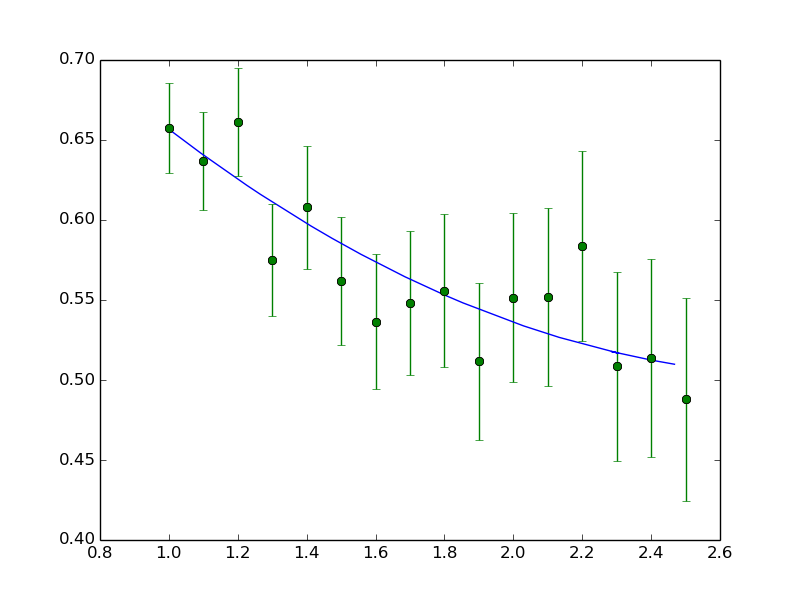
\includegraphics[width=0.8\textwidth]{cvgood.png}
\caption{ }
\end{figure}


\newpage
\section{Discussion}



The disadvantage of this method is that to find an accurate value for the specific heat capacity at constant volume is that the system has to be run for multiple temperatures.  

Truncation error comes from the algorithm used. 
Round-off error comes from how the data is stored. The Ercolessi program stores the data in single precision. The error analysis carried out in python was stored as double precision. The rounding error may be different for each machine the code is run on and the order of calculations matter.


for an isolated system the principle of equal 

Only the two body potential was used in this system, this is a reasonable approximation for Argon however is only useful when investigating isolated systems. The microcanonical ensemble investigated is computationally very quick to run however no systems in nature are truely isolated.   molecular simulation  

The simulation could be further expanded on by looking how the specific heat capacity of Argon varies with preasure. The Ercolessi program also writes out the pressure of the system at each time-step meaning all of the code written for the analysis would still be valid.

\newpage
\section{Conclusion}



Without block averaging the standard deviation of the mean of the internal energy is...less than the true standard deviation. 

The fluctuation formula method represents more flexibility in the properties of the system we can measure. 





\section{References}





 \begin{figure} [!ht]
 	\centering
 		\captionof{table} {How the step size effects the runtime and accuracy of the second and fourth order Runge-Kutta methods. The time command was used in the terminal to time how long the code took to execute. } \label{tab:title}
 		\begin{tabular}{| l | l | l | l | l |}
 			\hline
 			Step size, h & 2nd order R-K & Time (S) & 4th order R-K & Time (S) \\ \hline
 			0.1 & 5.1557273406861128  & 0.000 & 5.1939950699654398 & 0.000 \\ \hline
 			0.01 & 5.4184589256858491  & 0.000 & 5.4188564181985628 & 0.000 \\ \hline
 			0.001 & 5.4414584739981695  & 0.012 & 5.4414624508610689 & 0.016 \\ \hline
 			0.0001 & 5.4437124110825561  & 0.128 & 5.4437124508623658 & 0.168 \\ \hline
 			0.00001 & 5.4439374504402318  & 1.244 & 5.4439374508555876 & 1.690 \\ \hline
 			0.000001 & 5.4439598445085711  & 12.66 & 5.4439598445085711 & 16.86 \\ \hline
 		\end{tabular}
 		\bigskip 
 \end{figure}


\begin{itemize}
	\item 

\end{itemize}




\end{addmargin}
\end{document}